% Drawing 154/06-15 -- folder 154, batch 06, archive page 117 (PDF page 118).
% Transcription: dessin en couleur : un hexagone bordé de vert clair et de noir, rempli de courbes rouges qui s'entrecroisent
% Kind: hexagon filled with crossing red curves. Method 2 (schematic redraw from the facsimile). Status: partial.
% Notes: A hexagon bordered in light green and black, filled with red curves that cross one another (about ten strands, schematic; several run vertically to the bottom side). Read from the page view. Still differs from the facsimile: A hexagon bordered in light green and black, filled with red curves that cross one another (about ten strands, schematic; several run vertically to the bottom side).
% Coordinates: 1 unit = 1 mm = 1/100 of the crop width (bbox in page fractions: [0.624, 0.243, 0.773, 0.339]).
% Redrawn by Claude (claude-opus-5-5), issue #73, 2026-11-07; not checked by a human; not compiled (no TeX in the session).
% Revised by Claude (claude-opus-5-5) 2026-11-09 (issue #128) after Michel's check: vertices snapped to exact intersections (drawn points on their lines, meeting ends on the stroke they meet, near-concurrent lines through one computed point, curve ends on their rim); labels at \small as in folder 80 batch 3. Status: partial.
% Rights: reproduces part of the work -- behind RENDER_TRANSCRIPTS, never published by itself.
\documentclass[tikz,border=3pt]{standalone}
\usepackage{amsmath,amssymb}
\usetikzlibrary{patterns,arrows.meta}
\tikzset{Or/.style={orange!90!black}, Ye/.style={yellow!80!orange}, Lg/.style={green!60!black!70}, Dg/.style={green!45!black}, Br/.style={brown!80!black}, Rd/.style={red!85!black}, Bl/.style={blue!70!black}, Gy/.style={black!40}, pencil/.style={black!45}, struck/.style={black!35}, mark/.style={circle,draw,inner sep=1.3pt}, pt/.style={circle,fill,inner sep=0.9pt}, opt/.style={circle,draw,fill=white,inner sep=1.1pt}}
\begin{document}
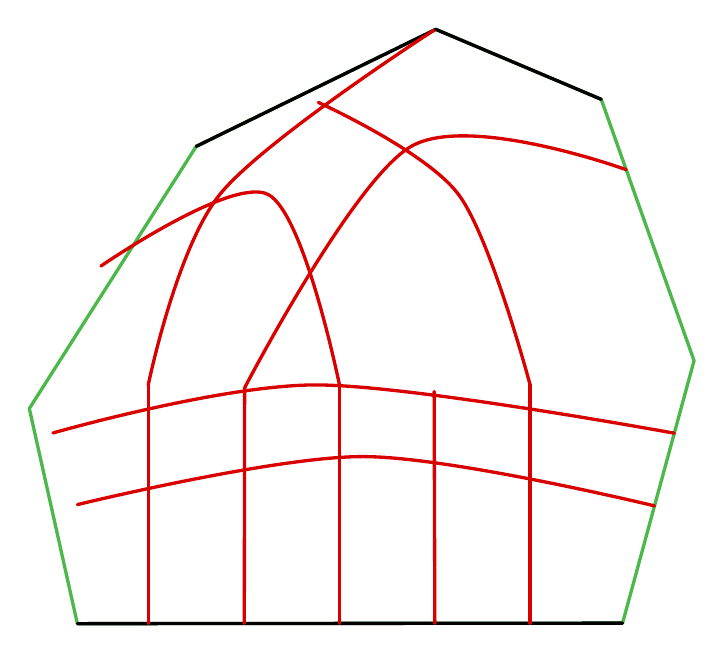
\begin{tikzpicture}[x=1mm,y=1mm,line cap=round,line join=round,font=\scriptsize]
\draw[Lg,very thick] (9.1,-54.5) -- (30.3,-21.2) -- (60.72,-6.34) -- (81.73,-15.23) -- (93.52,-48.42) -- (84.44,-81.75) -- (15.2,-81.82) -- cycle;
\draw[very thick] (30.3,-21.2) -- (60.72,-6.34) -- (81.73,-15.23);
\draw[very thick] (15.2,-81.82) -- (84.44,-81.75);
\draw[Rd,very thick] (24.2,-51.5) -- (24.2,-81.81);
\draw[Rd,very thick] (36.44,-51.87) -- (36.4,-81.8);
\draw[Rd,very thick] (48.5,-51.56) -- (48.5,-81.79);
\draw[Rd,very thick] (60.51,-52.34) -- (60.6,-81.78);
\draw[Rd,very thick] (72.7,-51.5) -- (72.7,-81.76);
\draw[Rd,very thick] plot[smooth, tension=0.55] coordinates {(12.1,-57.6) (45.5,-51.5) (91.01,-57.63)};
\draw[Rd,very thick] plot[smooth, tension=0.55] coordinates {(15.2,-66.7) (51.5,-60.6) (88.5,-66.86)};
\draw[Rd,very thick] plot[smooth, tension=0.55] coordinates {(24.2,-51.5) (33.3,-27.3) (60.48,-6.46)};
\draw[Rd,very thick] plot[smooth, tension=0.55] coordinates {(72.7,-51.5) (63.6,-27.3) (45.8,-15.62)};
\draw[Rd,very thick] plot[smooth, tension=0.55] coordinates {(36.44,-51.87) (57.6,-21.2) (84.9,-24.16)};
\draw[Rd,very thick] plot[smooth, tension=0.55] coordinates {(48.5,-51.56) (39.4,-27.3) (18.2,-36.4)};
\end{tikzpicture}
\end{document}
